\documentclass[aspectratio=169,10pt]{beamer}

% ----------------------------------------------------------------------
% Theme & Typography
% ----------------------------------------------------------------------
\usetheme{metropolis}
\usepackage{appendixnumberbeamer}
\usepackage{booktabs}
\usepackage{amsmath,amssymb}
\usepackage{microtype}
\usepackage{graphicx}
\usepackage{tikz}
\usetikzlibrary{arrows.meta, positioning, shapes.geometric, shapes.arrows, backgrounds, fit, calc, shadows}

% ----------------------------------------------------------------------
% Custom Oceanic Color Palette
% ----------------------------------------------------------------------
\definecolor{OceanDark}{RGB}{11, 37, 69}       % Deep Navy / Abyssal
\definecolor{OceanMedium}{RGB}{19, 64, 116}    % Oceanic Blue
\definecolor{OceanTeal}{RGB}{0, 119, 145}      % Coastal / Marine Teal
\definecolor{SeagrassGreen}{RGB}{34, 112, 70}  % Seagrass Canopy Green
\definecolor{CoralAccent}{RGB}{217, 83, 79}     % Coral / Alert red-orange
\definecolor{BgLight}{RGB}{250, 251, 252}      % Clean white-gray

% Apply colors to Metropolis
\setbeamercolor{normal text}{fg=OceanDark, bg=BgLight}
\setbeamercolor{alerted text}{fg=CoralAccent}
\setbeamercolor{example text}{fg=SeagrassGreen}
\setbeamercolor{frametitle}{fg=white, bg=OceanDark}
\setbeamercolor{title separator}{fg=OceanTeal}
\setbeamercolor{progress bar}{fg=OceanTeal, bg=OceanDark!20}
\setbeamercolor{block title}{fg=white, bg=OceanMedium}
\setbeamercolor{block body}{fg=OceanDark, bg=OceanMedium!10}
\setbeamercolor{block title alerted}{fg=white, bg=CoralAccent}
\setbeamercolor{block body alerted}{fg=OceanDark, bg=CoralAccent!10}
\setbeamercolor{block title example}{fg=white, bg=SeagrassGreen}
\setbeamercolor{block body example}{fg=OceanDark, bg=SeagrassGreen!10}

% Slide numbering
\setbeamertemplate{frame numbering}[fraction]

% Adjust block padding so block text does not touch borders
\makeatletter
\setlength{\metropolis@blocksep}{1.1ex}
\setlength{\metropolis@blockadjust}{0.3ex}
\makeatother

% Bottom citations / references for slides anchored to the absolute bottom
\newcommand{\slidecite}[1]{%
  \begin{tikzpicture}[remember picture, overlay]
    \node[anchor=south west, inner sep=0pt, xshift=0.8cm, yshift=0.25cm] at (current page.south west) {%
      \begin{minipage}{\dimexpr\paperwidth-2.6cm\relax}
        {\color{OceanDark!25}\rule{\linewidth}{0.4pt}}\par\vspace{1.5pt}%
        {\raggedright\tiny\color{OceanDark!75}#1\par}%
      \end{minipage}%
    };
  \end{tikzpicture}%
}

% ----------------------------------------------------------------------
% Presentation Metadata
% ----------------------------------------------------------------------
\title{Artificial Intelligence Applied to the Mapping and Monitoring of Seagrass Meadows}
\subtitle{From Classical Pixels to Foundation Models --- and the Challenge of Dataset Shift}
\author{\textbf{Pablo González}$^{1}$ \and \textbf{Fernando García-González}$^{2}$}
\institute{
  $^{1}$Artificial Intelligence Center (AIC), Universidad de Oviedo\\
  $^{2}$Instituto Español de Oceanografía (IEO-CSIC)
}
\date{CartoGrass Workshop --- 2026}

% ----------------------------------------------------------------------
\begin{document}

% ======================================================================
% SLIDE 1: Title
% ======================================================================
\begin{frame}[plain]
  \titlepage
\end{frame}

% ======================================================================
% SLIDE 2: Introduction & The Monitoring Bottleneck
% ======================================================================
\begin{frame}{Introduction \& The Monitoring Bottleneck}
  \begin{columns}[T]
    \begin{column}{0.54\textwidth}
      \begin{itemize}
        \item \textbf{What is this talk about?} Understanding the role of AI in seagrass monitoring.
        \item \textbf{From the past to the future:} Evolution of AI in seagrass mapping: from old fashioned techniques to modern approaches.
        \item \textbf{Are there any challenges?} Yes, there are!
      \end{itemize}
      \vspace{0.1cm}
      \begin{alertblock}{The Operational Bottleneck}
        In situ sampling and manual labelling are \textbf{costly, localized, and temporally sparse}.
      \end{alertblock}
    \end{column}
    \begin{column}{0.44\textwidth}
      \centering
      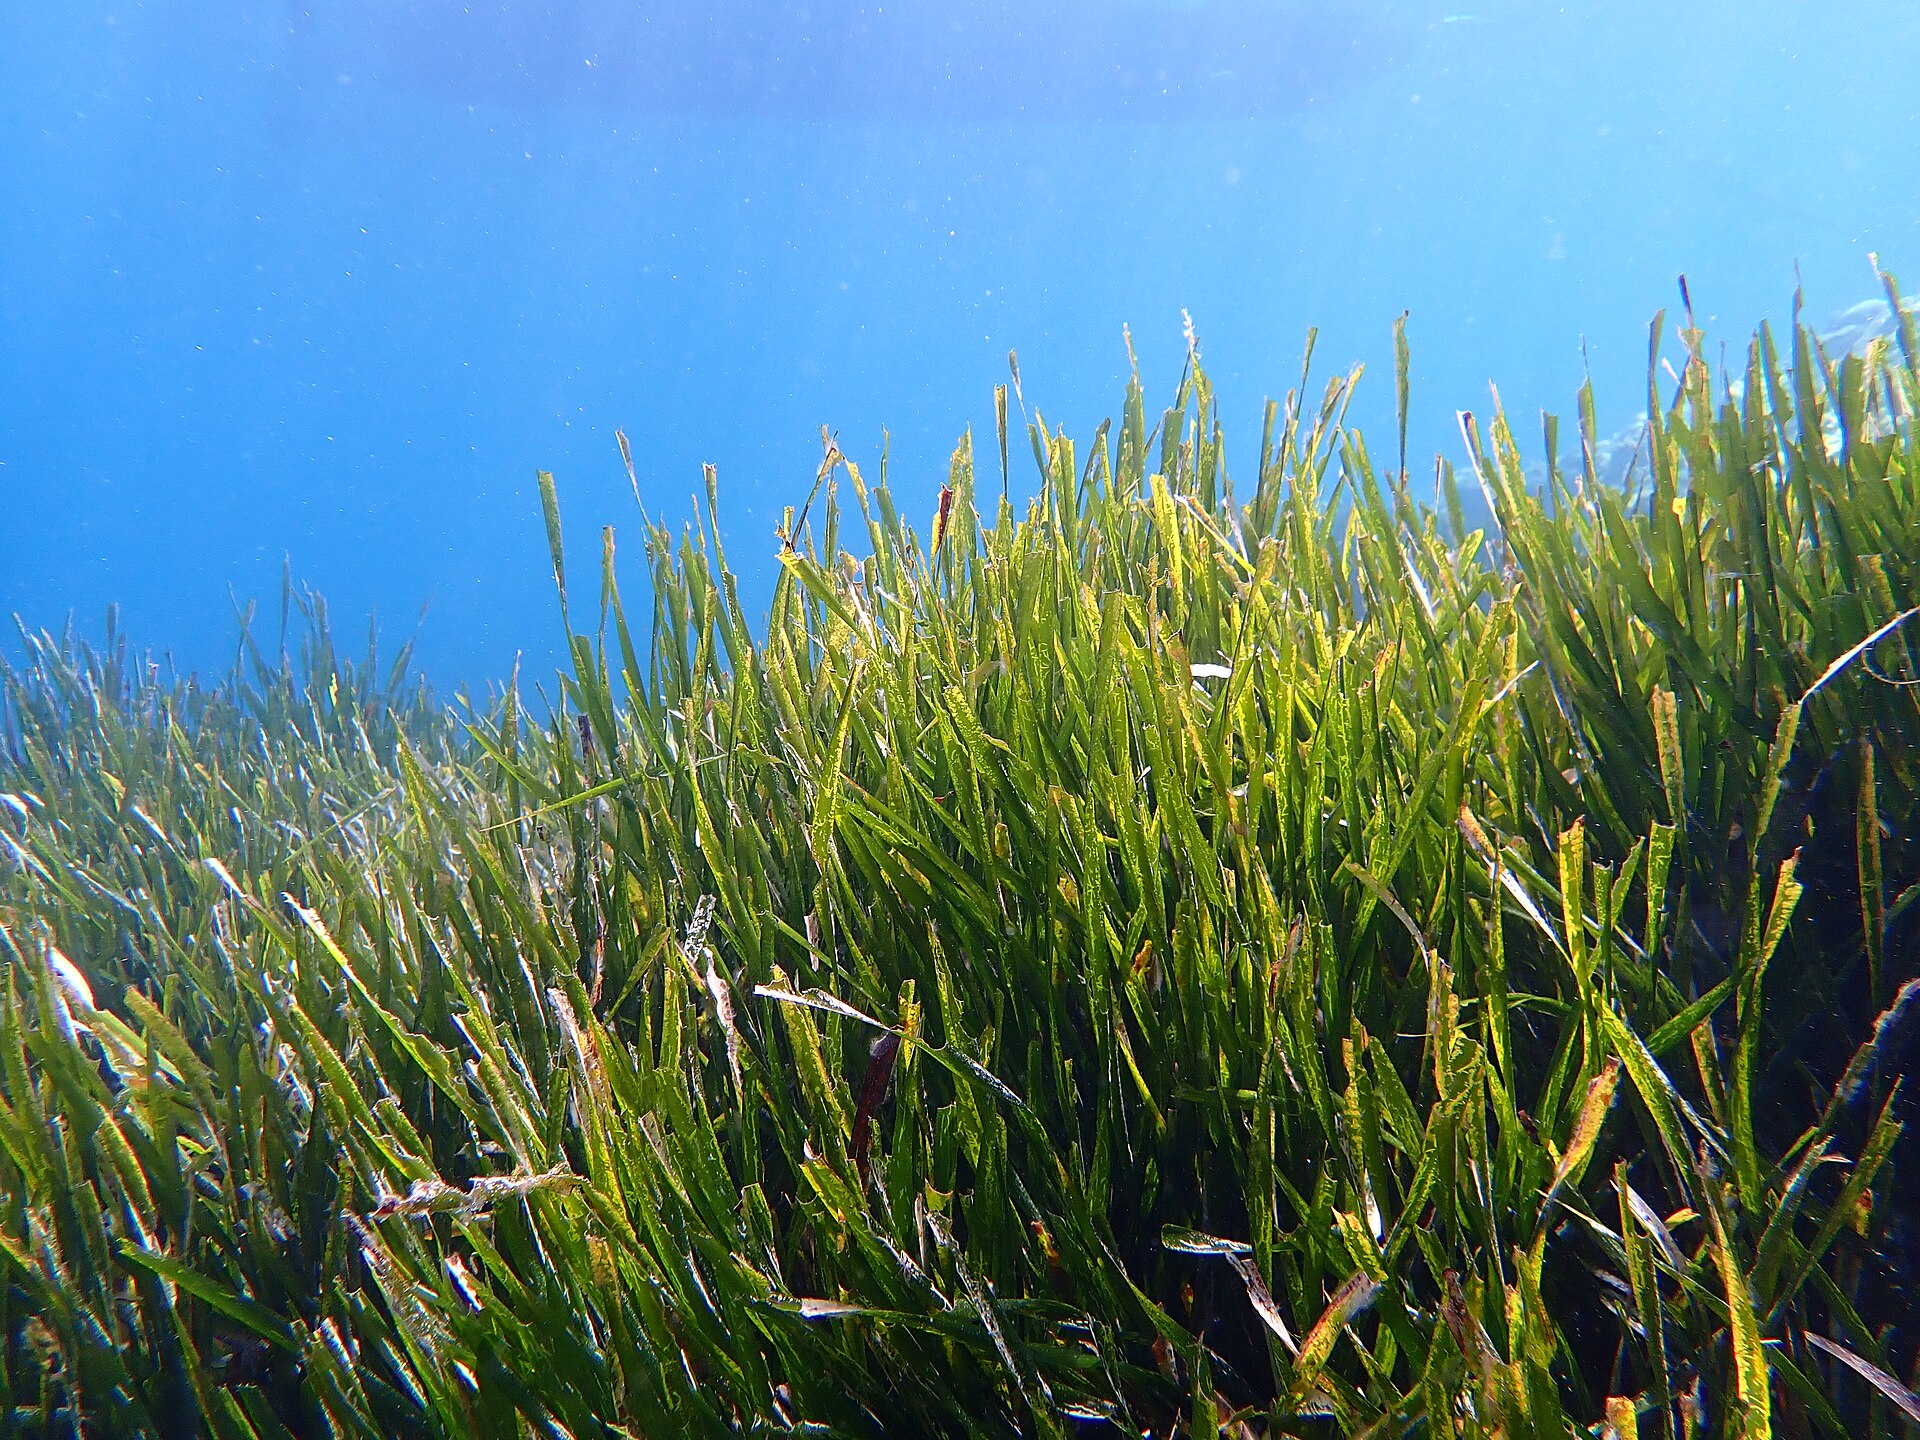
\includegraphics[width=\linewidth, height=4cm, keepaspectratio]{figures/posidonia_underwater.png}\\[3pt] 
      \textit{\scriptsize Submerged seagrass canopy in coastal waters (e.g. \textit{Posidonia oceanica}).}\par
      \vspace{0.3cm}
    \end{column}
  \end{columns}
  \Large \centering \textit{How can AI turn sparse observation into continuous, operational monitoring?}
\end{frame}

% ======================================================================
% SLIDE 3: The Multi-Source Data Landscape
% ======================================================================
\begin{frame}{The Multi-Source Remote Sensing Landscape}
  \begin{columns}[T]
    \begin{column}{0.48\textwidth}
      \centering
      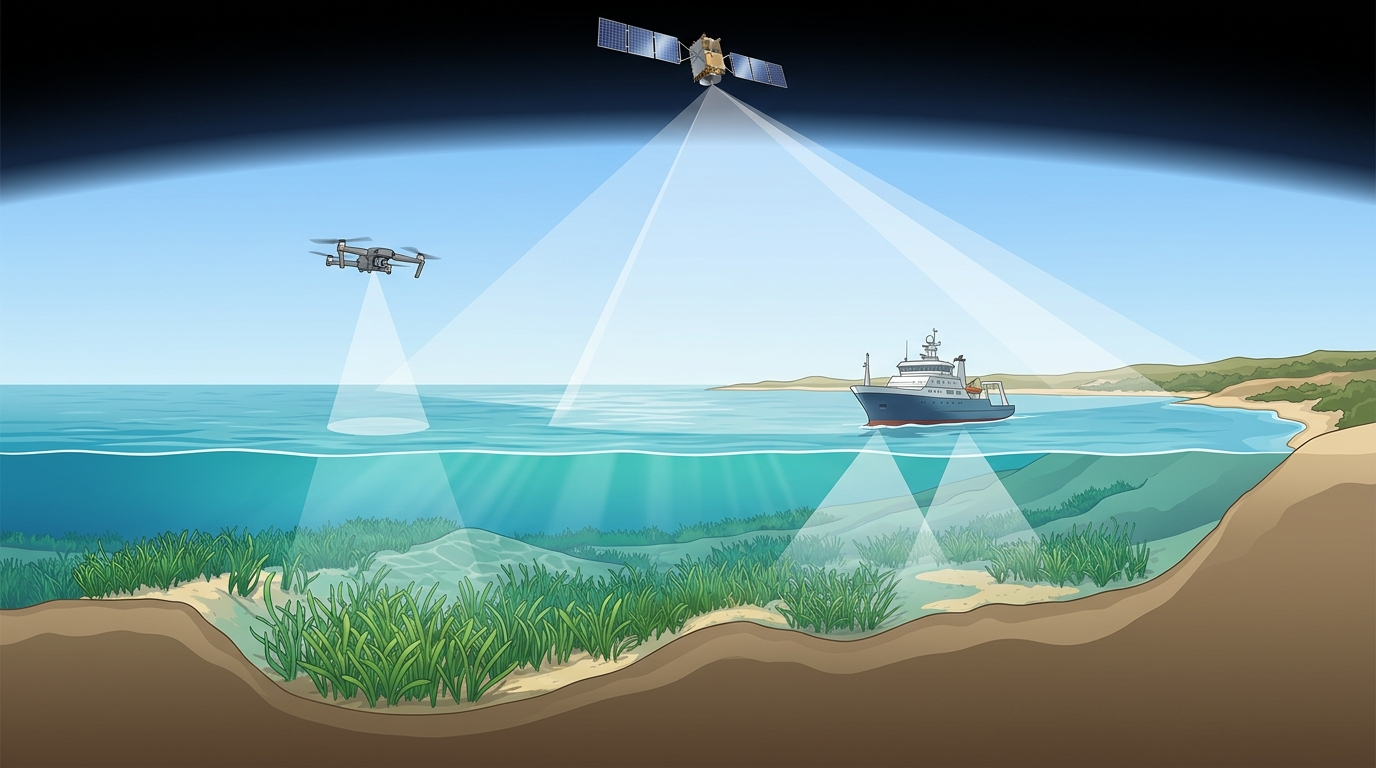
\includegraphics[width=\linewidth, height=4.4cm, keepaspectratio]{figures/sensing_platforms.jpg}\\[3pt]
      \textit{\scriptsize Multi-tier observation: Satellites, Drones, Vessels, \& Seafloor.}
    \end{column}
    \begin{column}{0.50\textwidth}
      \textbf{So many sources of data:}
      \begin{itemize}
        \item \textbf{Satellites (Sentinel-2, Landsat):}\newline
        {\footnotesize Global or nearly global coverage; 5-day revisit; 10m resolution; historical archives ($>30$ yrs).}
        \item \textbf{Drones (UAVs):}\newline
        {\footnotesize Centimetric detail (1--5\,cm); rapid deployment; local surveys.}
        \item \textbf{Underwater Vision (ROV/AUV/Drop-cam):}\newline
        {\footnotesize Millimetric in situ validation. }
        \item \textbf{Acoustics (MBES, Side-Scan Sonar):}\newline
        {\footnotesize High-resolution bathymetry and seafloor mapping.}
      \end{itemize}
    \end{column}
  \end{columns}
\end{frame}

% ======================================================================
% SLIDE 4: THE CENTRAL PLOT: The Three Eras of AI in Seagrass Mapping
% ======================================================================
\begin{frame}{Evolution: Three Eras of Seagrass Automated Mapping}
  \centering
  \begin{tikzpicture}[
    scale=0.88, every node/.style={transform shape},
    card/.style={
      rectangle, rounded corners=6pt,
      minimum width=4.3cm, text width=4.1cm, minimum height=4.3cm,
      inner sep=6pt, align=left, drop shadow={opacity=0.25, shadow xshift=2pt, shadow yshift=-2pt}
    },
    chevron/.style={
      single arrow, draw=OceanTeal!90, fill=OceanTeal!30, line width=1.1pt,
      minimum height=0.95cm, minimum width=0.46cm,
      single arrow head extend=2mm, inner sep=0pt,
      drop shadow={opacity=0.2, shadow xshift=1pt, shadow yshift=-1pt}
    }
  ]
    % Era 1 Card
    \node[card, fill=OceanMedium!10, draw=OceanMedium, line width=1.3pt] (era1) at (0, 1.35) {
      {\centering \textbf{\small Era 1: Pixel-by-Pixel}\par}
      \vspace{1.5pt}
      {\centering \textit{\scriptsize Spectral Paradigm (2000--)}\par}
      \vspace{4pt}\hrule height 0.6pt\vspace{5pt}
      \scriptsize
      $\bullet$ \textbf{Input:} Each of the pixels in the image\\[2.5pt]
      $\bullet$ \textbf{Context:} No spatial context\\[2.5pt]
      $\bullet$ \textbf{Methods:} MLP, SVM, Random Forest, etc\\[2.5pt]
      $\bullet$ \textbf{Limitation:} Sensitive to noise; ignores spatial patterns.
    };

    % Era 2 Card
    \node[card, fill=SeagrassGreen!10, draw=SeagrassGreen, line width=1.3pt] (era2) at (5.3, 1.35) {
      {\centering \textbf{\small Era 2: Deep Learning}\par}
      \vspace{1.5pt}
      {\centering \textit{\scriptsize Spatial Context Paradigm (2015--)}\par}
      \vspace{4pt}\hrule height 0.6pt\vspace{5pt}
      \scriptsize
      $\bullet$ \textbf{Input:} Image tensor\\[2.5pt]
      $\bullet$ \textbf{Context:} Learns spatial-spectral patterns\\[2.5pt]
      $\bullet$ \textbf{Features:} Hierarchical features (edges, textures, etc.)\\[2.5pt]
      $\bullet$ \textbf{Methods:} CNNs, U-Net, ViTs, etc.\\[2.5pt]
      $\bullet$ \textbf{Limitation:} Needs task-specific labels
    };

    % Era 3 Card
    \node[card, fill=OceanTeal!10, draw=OceanTeal, line width=1.3pt] (era3) at (10.6, 1.35) {
      {\centering \textbf{\small Era 3: Foundation Models}\par}
      \vspace{1.5pt}
      {\centering \textit{\scriptsize Large-Scale Pre-training (2020s--)}\par}
      \vspace{4pt}\hrule height 0.6pt\vspace{5pt}
      \scriptsize
      $\bullet$ \textbf{Input:} Image tensor\\[2.5pt]
      $\bullet$ \textbf{Context:} Patterns learned across large datasets\\[2.5pt]
      $\bullet$ \textbf{Pre-training:} Uses unlabelled imagery data\\[2.5pt]
      $\bullet$ \textbf{Models:} Prithvi, SatMAE, TerraMind, etc.\\[2.5pt]
      $\bullet$ \textbf{Adaptation:} Linear probes, fine-tuning, few-shot
    };

    % High-impact graphical chevron arrows between cards
    \node[chevron] (arrow1) at ($(era1.east)!0.5!(era2.west) + (0,-0.4)$) {};
    \node[chevron] (arrow2) at ($(era2.east)!0.5!(era3.west) + (0,-0.4)$) {};

    % Clean pill badges above chevrons
    \node[font=\tiny\bfseries, color=OceanMedium, fill=white, draw=OceanMedium!60, line width=0.7pt, rounded corners=2.5pt, inner sep=2pt, drop shadow={opacity=0.15}] 
      at ($(arrow1) + (0, 0.65)$) {+ Context};
    \node[font=\tiny\bfseries, color=OceanTeal, fill=white, draw=OceanTeal!60, line width=0.7pt, rounded corners=2.5pt, inner sep=2pt, drop shadow={opacity=0.15}] 
      at ($(arrow2) + (0, 0.65)$) {+ Pre-train};

    % -------------------------------------------------------------
    % BIG BOTTOM ARROWS / RIBBONS (Shifted down via scope)
    % -------------------------------------------------------------
    \begin{scope}[yshift=-0.8cm]
      % Big Arrow 1: Increasing Context (pointing right)
      \fill[SeagrassGreen, rounded corners=3pt, drop shadow={opacity=0.2}] (-2.0, -1.30) rectangle (12.1, -0.90);
      \fill[SeagrassGreen, drop shadow={opacity=0.2}] (12.1, -0.75) -- (12.7, -1.10) -- (12.1, -1.45) -- cycle;
      \node[font=\footnotesize\bfseries, color=white] at (5.1, -1.10) {
        Increasing Spatial \& Semantic Context 
      };

    \end{scope}

  \end{tikzpicture}
\end{frame}

% ======================================================================
% SLIDE 5: Era 1: Pixel-by-Pixel Classification
% ======================================================================
\begin{frame}{Era 1: The Classical Pixel-by-Pixel Workflow}
  \begin{columns}[T]
    \begin{column}{0.5\textwidth}
      \textbf{Core Assumption:}
      \begin{itemize}
        \item Each pixel vector $\mathbf{x} \in \mathbb{R}^B$ is treated as an independent statistical sample.
        \item The spatial coordinates of the pixel are ignored.
        \item The context of the pixel is not used to inform the classification.
      \end{itemize}
      \vspace{0.15cm}
      \textbf{Advantages:}
      \begin{itemize}
        \item Simple and fast to implement.
        \item Publicly available libraries for typical classifiers.
        \item Works well for large, homogeneous meadows with clear spectral signatures.
      \end{itemize}
    \end{column}
    \begin{column}{0.48\textwidth}
      \begin{block}{Traditional Classifiers}
        \begin{itemize}
          \item \textbf{Multilayer Perceptron (MLP):} A feedforward neural network with multiple layers.
          \item \textbf{Support Vector Machines (SVM):} Maximum-margin kernel hyperplanes.
          \item \textbf{Random Forest (RF):} Ensemble of decision trees; the dominant baseline.
        \end{itemize}
      \end{block}
      \vspace{0.1cm}
      \small Standard pipeline: Sentinel-2/Landsat + field points $\rightarrow$ Random Forest pixel classification.
    \end{column}
  \end{columns}
\end{frame}



% ======================================================================
% SLIDE 7: Why Era 1 Hit a Ceiling (Limitations)
% ======================================================================
\begin{frame}{Why Era 1 Hit a Plateau: The Pixel Bottleneck}
  \begin{columns}[T,onlytextwidth]
    \begin{column}{0.32\textwidth}
      \begin{alertblock}{1. Spatial Blindness}
        A single pixel has zero context:
        \begin{itemize}
          \item Ignores texture and shape, confusing rock or algae with seagrass.
          \item Produces fragmented, noisy maps.
        \end{itemize}
      \end{alertblock}
    \end{column}
    
    \begin{column}{0.32\textwidth}
      \begin{alertblock}{2. Mixed Pixels}
        At 10--20\,m resolution:
        \begin{itemize}
          \item Meadow edges mix seagrass with bare sand, mud, or rock.
          \item Hard classifiers force an unrealistic binary (0/1) choice.
        \end{itemize}
      \end{alertblock}
    \end{column}
    
    \begin{column}{0.32\textwidth}
      \begin{alertblock}{3. Water Noise}
        Single pixels are fragile:
        \begin{itemize}
          \item Waves, sun glint, and turbidity easily distort individual spectra.
          \item Triggers false alarms of meadow loss or gain over time.
        \end{itemize}
      \end{alertblock}
    \end{column}
  \end{columns}

  \vspace{0.3cm}
\end{frame}

% ======================================================================
% SLIDE 8: Era 2: Why Spatial Context Matters (Pixel vs Patch)
% ======================================================================
\begin{frame}{Era 2: Why Spatial Context Matters --- From Pixels to Patches}
  \centering
  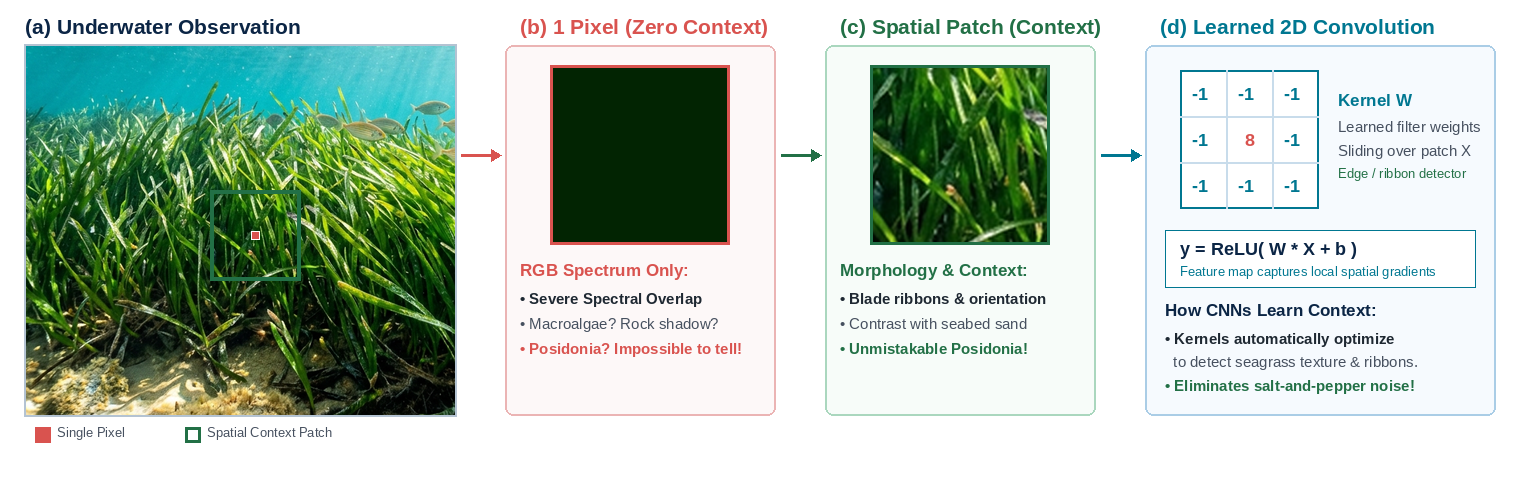
\includegraphics[width=\textwidth, height=3.55cm, keepaspectratio]{figures/pixel_vs_patch_context.png}
  
  \vspace{0.15cm}
  \begin{columns}[T]
    \begin{column}{0.48\textwidth}
      \textbf{The Single Pixel Dilemma (Era 1):}
      \begin{itemize}
        \item Isolated spectral vector $\mathbf{x} \in \mathbb{R}^B$ has severe class overlap (seagrass vs. macroalgae vs. shadow).
        \item Zero structural awareness.
      \end{itemize}
    \end{column}
    \begin{column}{0.48\textwidth}
      \textbf{The Deep Learning Revolution (Era 2):}
      \begin{itemize}
        \item Convolutional Neural Networks (CNNs) are able to learn spatial-spectral patterns directly from image patches.
        \item They were invented more than 35 years ago, and have been widely used in computer vision since 2012.
      \end{itemize}
    \end{column}
  \end{columns}
\end{frame}

\begin{frame}{From Patch Classification to Segmentation (U-Net)}
  \centering
  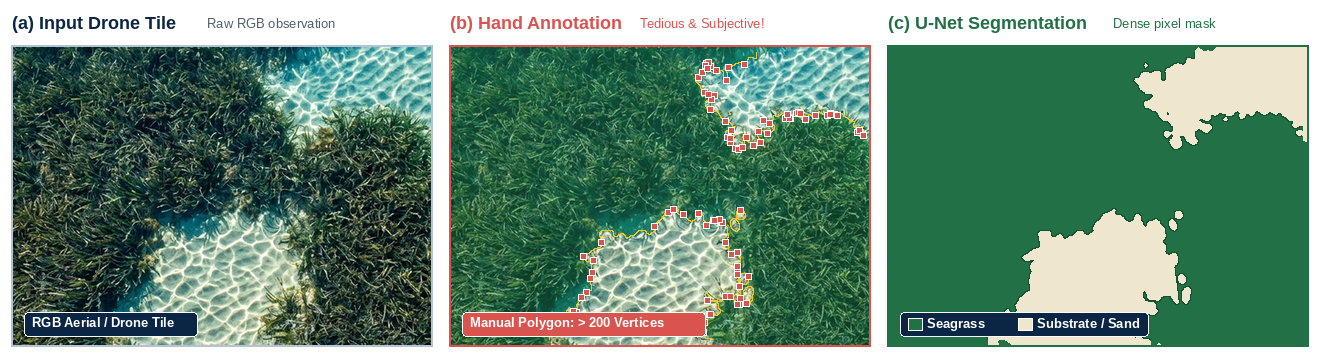
\includegraphics[height=1.95cm, keepaspectratio]{figures/seagrass_segmentation_unet.png}
  
  \vspace{0.05cm}
  \begin{columns}[T]
    \begin{column}{0.48\textwidth}
      \textbf{What Segmentation Solves:}
      \begin{itemize}\setlength{\itemsep}{1.2pt}
        \item \textbf{End-to-End Mapping:} Direct transformation of $H \times W$ tile $\rightarrow$ $H \times W$ habitat mask in one forward pass (no sliding patch artifacts).
        \item \textbf{Processing images at once: } U-Net like networks can process entire tiles at once, capturing global context.
        \item \textbf{What's a U-Net?:} A U shaped deep learning architecture with encoder-decoder structure and skip connections.
      \end{itemize}
    \end{column}
    \begin{column}{0.50\textwidth}
        \textbf{Labelling problem:}:
        \begin{itemize}\setlength{\itemsep}{1pt}
          \item \textbf{Extreme Manual Effort:} Tracing hundreds of polygon vertices in a image is very time consuming and difficult.
          \item \textbf{Limited Coverage:} Dense annotations are often only available for small areas, limiting model generalization.
          \item \textbf{Road to Era 3:} These problems motivate the use of self-supervised learning and foundation models.
        \end{itemize}
    \end{column}
  \end{columns}
\end{frame}


\begin{frame}{Era 3: Foundation Models: Learning Without Labels}
\vspace{0.1cm}
\begin{alertblock}{The Marine Label Bottleneck}
  Annotating underwater imagery is expensive and time-consuming,
  while vast amounts of satellite and marine imagery remain unlabeled.
\end{alertblock}

\begin{columns}[T,onlytextwidth]
  \begin{column}{0.48\textwidth}
    \begin{block}{Large Language Models\\(ChatGPT, Gemini, etc)}
      \centering
      \textbf{Predict the next token}

      \vspace{0.08cm}
      Read previous words;\\
      predict the next one: \textcolor{blue}{\textbf{?}}

      \vspace{0.08cm}
      \footnotesize
      \textit{Training data:} enormous text corpora\\
      collected from web, books, etc.
    \end{block}
  \end{column}

  \begin{column}{0.48\textwidth}
    \begin{exampleblock}{Earth Observation Models\\(Prithvi, TerraMind, etc)}
      \centering
      \textbf{Predict masked image patches}

      \vspace{0.08cm}
      Observe surrounding patches;\\
      reconstruct the hidden region.

      \vspace{0.08cm}
      \footnotesize
      \textit{Training data:} massive collections of\\
      unlabeled satellite imagery.
    \end{exampleblock}
  \end{column}
\end{columns}

\vspace{0.1cm}
{\centering
  \Large
  \textbf{Self-supervised learning: learn from the data itself}\par
  \vspace{0.05cm}
  \footnotesize
  Pretrain on abundant unlabeled data; adapt to seagrass mapping
  with a much smaller set of labeled examples.\par
}

\end{frame}


\begin{frame}[t]{Foundation Models for Earth Monitoring}
\small

\begin{columns}[T,onlytextwidth]

\begin{column}{0.49\textwidth}
  \textbf{1. Earth Observation}

  \vspace{0.05cm}
  \begin{itemize}
    \setlength{\itemsep}{0.08cm}

    \item \textbf{Prithvi}\textsuperscript{\color{OceanTeal}[1]} / \textbf{SatMAE}
    \begin{itemize}
      \item \textit{Masked reconstruction}
      \item Reconstruct hidden satellite patches
      to learn spectral and spatial patterns.
    \end{itemize}

    \item \textbf{TerraMind}\textsuperscript{\color{OceanTeal}[2]}
    \begin{itemize}
      \item \textit{Cross-modal prediction}
      \item Predict missing geospatial modalities
      from optical, SAR and other observations.
    \end{itemize}
  \end{itemize}
\end{column}

\begin{column}{0.49\textwidth}
  \textbf{2. Promptable Segmentation}

  \vspace{0.05cm}
  \begin{itemize}
    \setlength{\itemsep}{0.08cm}

    \item \textbf{Segment Anything (SAM)}\textsuperscript{\color{OceanTeal}[3]}
    \begin{itemize}
      \item \textit{Prompt-to-mask prediction}
      \item Given a point or bounding box,
      predict the corresponding object mask.
    \end{itemize}
  \end{itemize}
\end{column}

\end{columns}


\slidecite{%
  \textsuperscript{[1]} Jakubik et al.\ (NASA/IBM), \textit{Foundation Models for Generalist Geospatial AI}, arXiv:2310.18660 (2023).\\[0.8pt]
  \textsuperscript{[2]} Jakubik et al., \textit{TerraMind: Large-Scale Generative Multimodality for Earth Observation}, IEEE/CVF ICCV, pp.~7383--7394 (2025).\\[0.8pt]
  \textsuperscript{[3]} Kirillov et al.\ (Meta AI), \textit{Segment Anything}, IEEE/CVF ICCV, pp.~4015--4026 (2023).%
}

\end{frame}

\begin{frame}{TerraMind in Practice: From Tiles to Spatial Embeddings}
  \centering
  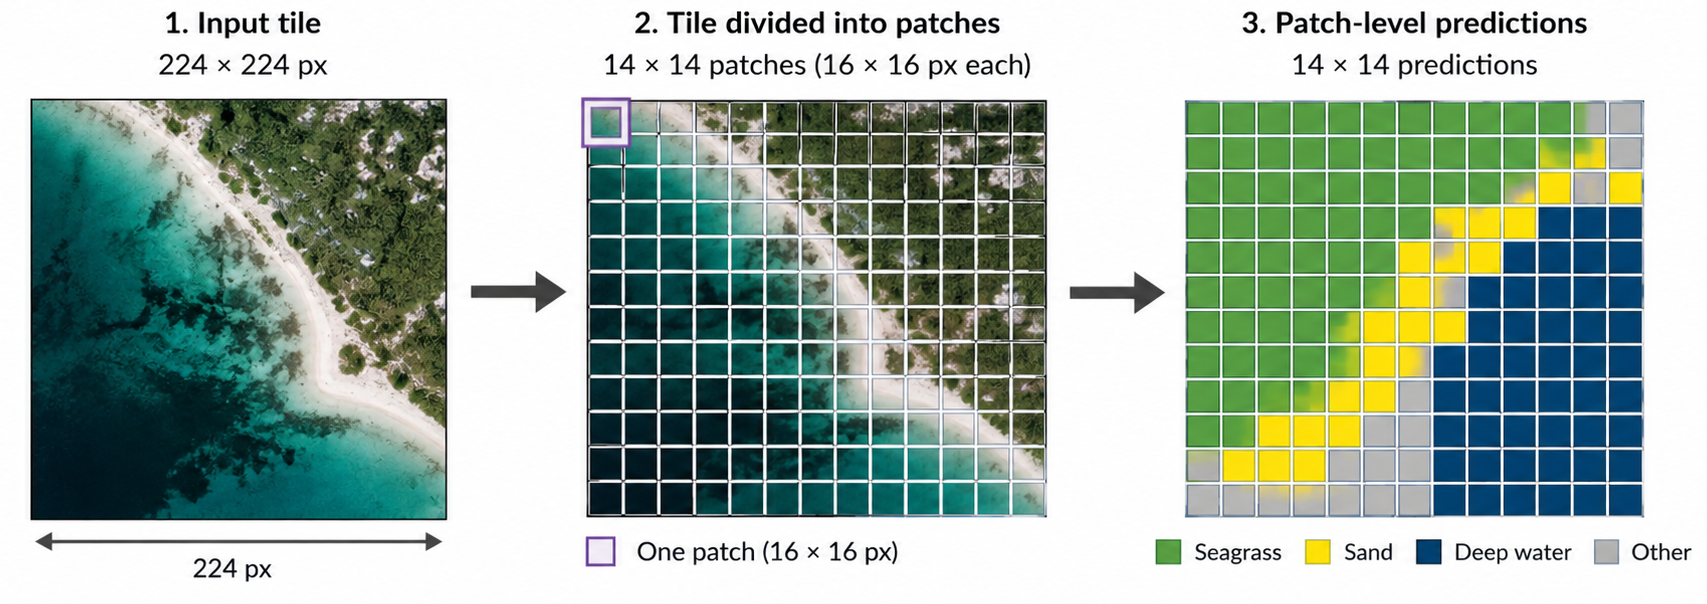
\includegraphics[height=3.5cm,keepaspectratio]
    {figures/terramind.png}
  \vspace{-0.2cm}

  \begin{columns}[T,onlytextwidth]
    \begin{column}{0.48\textwidth}
      \begin{block}{1. One Embedding per Tile}
        \footnotesize
        \begin{itemize}\setlength{\itemsep}{3pt}
          \item Input: a $224px\times224px$ satellite tile.
          \item TerraMind produces a single
            \textbf{tile-level representation}
            $\mathbf{z}\in\mathbb{R}^{d}$.
          \item Feed $\mathbf{z}$ to a standard
            classifier (e.g., Random Forest or SVM).
        \end{itemize}
        \vspace{0.05cm}
        \centering
        \textbf{Output:} tile-level habitat class
      \end{block}
    \end{column}

    \begin{column}{0.50\textwidth}
      \begin{exampleblock}{2. One Embedding per Patch}
        \footnotesize
        \begin{itemize}\setlength{\itemsep}{3pt}
          \item The tile contains $14\times14=196$
            spatial patches ($16\times16$ pixels each).
          \item TerraMind provides an
            \textbf{embedding per patch}.
          \item Train a classifier on each embedding
            to obtain a spatially detailed habitat map.
        \end{itemize}
        \vspace{0.05cm}
        \centering
        \textbf{Output:} patch-level habitat predictions
      \end{exampleblock}
    \end{column}
  \end{columns}
\end{frame}

\begin{frame}{The Three Eras: A Comparative Synthesis}
  \begin{center}
  \resizebox{0.98\textwidth}{!}{
  \begin{tabular}{lccc}
    \toprule
    \textbf{Dimension} & \textbf{Era 1: Pixel-by-Pixel} & \textbf{Era 2: Deep Learning} & \textbf{Era 3: Foundation Models} \\
    \midrule
    \textbf{Data Representation} & 1D vector $\mathbf{x} \in \mathbb{R}^B$ & 2D/3D patch $\mathbf{X} \in \mathbb{R}^{H \times W \times B}$ & Multi-modal latent representations \\
    \addlinespace[3pt]
    \textbf{Spatial Context} & Completely blind & Patch context & Global context \\
    \addlinespace[3pt]
    \textbf{Label Dependency} & High (per-pixel labels) & High (patches or dense masks) & Very low (few-shot / zero-shot) \\
    \addlinespace[3pt]
    \textbf{Core Methodologies} & SVM, Random Forest, etc & CNNs, ViTs, U-Nets, etc & Masked Autoencoders, BioCLIP, SAM, etc \\
    \addlinespace[3pt]
    \textbf{Main Limitation} & Sensitive to noise, no context & Data-hungry; overfitting on small surveys & Pre-training compute \\
    \bottomrule
  \end{tabular}
  }
  \end{center}
  \vspace{0.2cm}
  \begin{exampleblock}{The common blindspot}
    \centering
    All three eras share one critical vulnerability when taken out of the lab:
    
    \textbf{How do they handle data distribution changes?}
  \end{exampleblock}
\end{frame}

% ======================================================================
% SLIDE 14: The Reality Check: Lab to Sea
% ======================================================================
\begin{frame}{The Reality Check: Bringing AI from the Lab to the Sea}
  \begin{center}
    \large\textit{``Our model achieved 94\% F1-score on the test set...\\
    so why did it fail completely when deployed next summer?''}
  \end{center}
  \vspace{0.3cm}
  \begin{columns}[T,onlytextwidth]
    \begin{column}{0.48\textwidth}
      \begin{block}{The Standard ML Assumption}
        Training and test data are assumed\\
        independent and identically distributed:
        \begin{equation*}
          P_{\text{train}}(X, Y) \equiv P_{\text{test}}(X, Y)
        \end{equation*}
        $\Rightarrow$ \textbf{Stationary environment.}
      \end{block}
    \end{column}
    \begin{column}{0.48\textwidth}
      \begin{alertblock}{The Marine Reality}
        The ocean is an inherently dynamic,\\
        non-stationary coastal environment:
        \begin{equation*}
          P_{\text{train}}(X, Y) \neq P_{\text{deployment}}(X, Y)
        \end{equation*}
        $\Rightarrow$ \textbf{Dataset Shift.}
      \end{alertblock}
    \end{column}
  \end{columns}
  \vspace{0.3cm}
  \centering
  \textbf{In marine habitat mapping, high test accuracy is easy; transferability is hard.}
\end{frame}

% ======================================================================
% SLIDE 15: What is Dataset Shift?
% ======================================================================
\begin{frame}{Dataset Shift in Seagrass Monitoring}
  \small
  Standard classifiers assume data are i.i.d.\ ($P_{\text{train}} = P_{\text{test}}$). When this breaks down, \textbf{dataset shift} occurs, categorized into three fundamental types\textsuperscript{\color{OceanTeal}[1]}.
  
  By factorizing the joint distribution of the covariates $X$ and labels $Y$, we can express the relationship as:
  \begin{equation*}
    P(X, Y) = P(Y \mid X) \, P(X) = P(X \mid Y) \, P(Y)
  \end{equation*}

  \vspace{0.05cm}
  \begin{columns}[T,onlytextwidth]
    \begin{column}{0.32\textwidth}
      \begin{block}{Covariate Shift}
        $P(X)$ changes,\\
        $P(Y \mid X)$ remains fixed.
        \vspace{0.15cm}
        \footnotesize
        
        \textit{Example:} Water turbidity or illumination changes, but the true habitat boundary does not move.
      \end{block}
    \end{column}
    \begin{column}{0.32\textwidth}
      \begin{alertblock}{Concept Shift}
        $P(Y \mid X)$ changes,\\
        $P(X)$ could change.
        \vspace{0.15cm}
        \footnotesize

        \textit{Example:}  Accumulations of dead algae covering the bottom change how a living seagrass meadow looks.
      \end{alertblock}
    \end{column}
    \begin{column}{0.32\textwidth}
      \begin{exampleblock}{Prior Shift}
        $P(Y)$ changes,\\
        $P(X \mid Y)$ remains fixed.
        \vspace{0.15cm}
        \footnotesize

        \textit{Example:} Moving from a dense continuous reserve (70\% cover) to a fragmented urbanized bay (5\% cover).
      \end{exampleblock}
    \end{column}
  \end{columns}

  \slidecite{%
    \textsuperscript{[1]} Moreno-Torres et al., \textit{A unifying view on dataset shift in machine learning}, Pattern Recognition, 45(1), pp.~521--530 (2012).%
  }
\end{frame}


% ======================================================================
% SLIDE 17: Shift Vulnerability Across the Three Eras
% ======================================================================
\begin{frame}{How the Three Eras Behave Under Dataset Shift}
  \begin{columns}[T]
    \begin{column}{0.32\textwidth}
      \textbf{Era 1: Pixel Models}
      \begin{itemize}
        \item \textbf{Extremely fragile} to Covariate Shift: any illumination or turbidity change pushes the 1D spectrum out of the decision boundary.
        \item Requires constant per-scene manual re-calibration.
      \end{itemize}
    \end{column}
    \begin{column}{0.32\textwidth}
      \textbf{Era 2: Deep Learning}
      \begin{itemize}
        \item Context rejects local noise, but CNNs often suffer from \textbf{texture / domain shortcut learning}.
        \item Overfits to training water characteristics; silent, catastrophic failures on new unseen coasts.
      \end{itemize}
    \end{column}
    \begin{column}{0.32\textwidth}
      \textbf{Era 3: Foundation Models}
      \begin{itemize}
        \item Pre-trained on diverse global distributions: greater \textbf{latent robustness}.
        \item Contrastive pre-training enforces invariance to lighting and sensor quirks.
        \item Can still drift under localized Concept Shifts.
      \end{itemize}
    \end{column}
  \end{columns}
  \vspace{0.3cm}
  \begin{center}
    \textit{As models become more expressive, managing distribution shift becomes the true limiting factor for operational adoption.}
  \end{center}
\end{frame}


% ======================================================================
% SLIDE 19: Conclusions & The Road Ahead
% ======================================================================
\begin{frame}{Conclusions \& The Road Ahead}
  \begin{enumerate}
    \item \textbf{The Technological Leap:} Marine habitat mapping has transitioned from rigid, isolated spectral pixels (Era 1) to rich spatial-context deep architectures (Era 2), and now to self-supervised foundation models (Era 3).
    \vspace{0.15cm}
    \item \textbf{Bypassing the Label Bottleneck:} Foundation models pre-trained on planetary-scale Earth observation archives drastically reduce our dependence on prohibitive underwater field campaigns.
    \vspace{0.15cm}
    \item \textbf{The True Frontier is Dataset Shift:} Moving AI from academic benchmarks to operational public policy requires models that survive non-stationary oceans, seasonal canopy dynamics, and sensor migrations.
    \vspace{0.15cm}
    \item \textbf{Operational Principle:} \textit{Success is no longer measured by accuracy on a static test set, but by robustness to distribution shift across space and time.}
  \end{enumerate}
\end{frame}

% ======================================================================
% SLIDE 20: Thank You / Q&A
% ======================================================================
\begin{frame}[standout]
  \Large Thank You for Your Attention!\\[16pt]
  \normalsize
  \textbf{Artificial Intelligence Applied to the Mapping and Monitoring of Seagrass Meadows}\\[12pt]
  \small
  \textbf{Pablo González}$^{1}$ \quad \& \quad \textbf{Fernando García-González}$^{2}$\\[4pt]
  $^{1}$AIC, Universidad de Oviedo \quad $^{2}$IEO-CSIC\\[16pt]
  \textit{Questions \& Discussion}
\end{frame}

\end{document}
